\documentclass[12pt, a4paper, titlepage, oneside, abstract=true, toc=listof, toc=bibliography]{scrreprt}

\usepackage[utf8]{inputenc}
\usepackage{amsmath}
\usepackage{amsfonts}
\usepackage{amssymb}
\usepackage[titletoc]{appendix}
\usepackage[english]{babel}
\usepackage{caption}
\usepackage{graphicx}
\usepackage[colorlinks=true,urlcolor=blue,citecolor=red,linkcolor=red,bookmarks=true,linktoc=all,bookmarkstype=toc,bookmarksopen=true]{hyperref}
\usepackage{longtable}
\usepackage{natbib}
%\usepackage{biblatex}
\usepackage[intoc,english]{nomencl}
\usepackage{textcomp}
\usepackage{xpatch}
\usepackage{pdfpages}


\usepackage[acronym, toc, automake, nonumberlist]{glossaries}
% \newglossary[]{software}{sw}{ntn}{Notation}
% no hyperlinks for glossary entries
\newglossary*{software}{Glossary of Mentioned Software and Services}
\glsdisablehyper
\makeglossaries

%% Glossary of Mentioned Software and Services
%% A
\newglossaryentry{Academia}{type=software, name=Academia, description={\url{https://www.academia.edu/}}}
\newglossaryentry{AntConc}{type=software, name=AntConc, description={\url{}}}
\glsadd{AntConc}
%% B
\newglossaryentry{Bryn}{type=software, name=Bryn Mawr Classical Review, description={\url{ http://bmcr.brynmawr.edu/
}}}
\glsadd{Bryn}
%% C
\newglossaryentry{Catul}{type=software, name=Catul online, description={\url{}}}
\glsadd{Catul}
\newglossaryentry{Citavi}{type=software, name=Citavi, description={A reference management software. \url{https://www.citavi.com/en}}}
%% D
\newglossaryentry{DeepL}{type=software, name=DeepL, description={\url{}}}
\glsadd{DeepL}
\newglossaryentry{Dropbox}{type=software, name=Dropbox, description={\url{}}}
\glsadd{Dropbox}
\newglossaryentry{Excel}{type=software, name=Excel (Microsoft), description={\url{}}}
\glsadd{Excel}
%% G
\newglossaryentry{Germanistik.net}{type=software, name=Germanistik.net, description={\url{}}}
\glsadd{Germanistik.net}
\newglossaryentry{Gnomon}{type=software, name=Gnomon online, description={\url{https://www.chbeck.de/buecher/zeitschriften/gnomon/
}}}
\newglossaryentry{Google}{type=software, name=Google Scholar, description={\url{https://scholar.google.com}}}
%% J
\newglossaryentry{JSTOR}{type=software, name=JSTOR, description={\url{}}}
\glsadd{JSTOR}
%% L
\newglossaryentry{LAPh}{type=software, name=l'Année philologique online, description={\url{http://www.brepols.net/Pages/BrowseBySeries.aspx?TreeSeries=APH-O
}}}
\newglossaryentry{Latex}{type=software, name=\LaTeX, description={\url{}}}
\glsadd{Latex}
\newglossaryentry{LLTA_SW}{type=software, name=Library of Latin Texts, description={\url{}}}
\glsadd{LLTA_SW}
%% P
\newglossaryentry{Perseus}{type=software, name=Perseus, description={\url{}}}
\glsadd{Perseus}
%% S
\newglossaryentry{Stylo}{type=software, name=Stylo, description={\url{https://github.com/computationalstylistics/stylo}}}
\glsadd{Stylo}
%% T
\newglossaryentry{Thunderbird}{type=software, name=Mozilla Thunderbird, description={\url{}}}
\glsadd{Thunderbird}
\newglossaryentry{TLG_SW}{type=software, name=Thesaurus Linguae Graecae, description={\url{https://stephanus.tlg.uci.edu
}}}
\glsadd{TLG_SW}
\newglossaryentry{TLL_SW}{type=software, name=Thesaurus Linguae Latinae, description={\url{https://db.degruyter.com/databasecontent?dbid=tll&dbsource=%2Fdb%2Ftll&language=en
}}}
\glsadd{TLL_SW}
\newglossaryentry{Typegreek}{type=software, name=typegreek, description={\url{http://www.typegreek.com/
}}}
%% W
\newglossaryentry{Word}{type=software, name=Word (Microsoft), description={\url{}}}


%\newglossaryentry{}{type=software, name=, description={}}
%\newglossaryentry{}{type=software, name=, description={}}
%\newglossaryentry{}{type=software, name=, description={}}


%% Acronyms
\newacronym{DH}{DH}{Digital Humanities}
\newacronym{TLG}{TLG}{Thesaurus Linguae Graecae}
\newacronym{TLL}{TLL}{Thesaurus Linguae Latinae}
\newacronym{LLTA}{LLTA}{Library of Latin Texts}
\newacronym{BMCR}{BMCR}{Bryn Mawr Classical Review}
\newacronym{IP}{IP}{Information Practices}
\newacronym{IB}{IB}{Information Behavior}
\newacronym{APh}{APh}{l'Année philologique}

%zähler ohne kapitelnummern
\counterwithout{figure}{chapter}
\counterwithout{table}{chapter}

\begin{document}

%----------------------------------------------------------------------------------------
%	TITLE PAGE
%----------------------------------------------------------------------------------------

\begin{titlepage} % Suppresses displaying the page number on the title page and the subsequent page counts as page 1
	\newcommand{\HRule}{\rule{\linewidth}{0.5mm}} % Defines a new command for horizontal lines, change thickness here
	
	\center % Centre everything on the page
	
	%------------------------------------------------
	%	Headings
	%------------------------------------------------
	
	\textsc{\LARGE Humboldt University of Berlin}\\[1.0cm] % Main heading such as the name of your university/college
	
	\textsc{\Large Institute for Library and Information Science}\\[0.5cm] % Major heading such as course name
	
	
	%------------------------------------------------
	%	Logo
	%------------------------------------------------
	
	\vfill
	
\includegraphics[width=0.2\textwidth]{husiegel_bw_op.eps}\\[1cm] % Include a department/university logo - this will require the graphicx package

	%\textsc{\large Minor Heading}\\[0.5cm] % Minor heading such as course title
	
	%------------------------------------------------
	%	Title
	%------------------------------------------------
	
	%\HRule\\[1cm]
	\vfill
	{\large\textsc{Seeking Research Software. A Qualitative Study of Humanities Scholars' Information Practices.}}\\[0.8cm] % Title of your document
	{\textsc{Master's Thesis in the Postgraduate Master's Program in Library and Information Science by Distance Learning}}\\
	%\HRule\\[3.6cm]
	\vfill	
	
	%------------------------------------------------
	%	Author(s)
	%------------------------------------------------
	
			\large
			\textsc{Ronny Gey}\\[0.8cm]% Your name
			
	%------------------------------------------------
	%	Supervisor(s)
	%------------------------------------------------
	
			\textsc{Supervisors:\\ Prof. Rebecca D. Frank, Ph.D.\\Prof. Dr. Wolfram Horstmann}
	
	
	%------------------------------------------------
	%	Date
	%------------------------------------------------
	
	\vfill\vfill\vfill % Position the date 3/4 down the remaining page
	
	{\textsc{Leipzig, \today}} % Date, change the \today to a set date if you want to be precise
		 
	%----------------------------------------------------------------------------------------
	
	\vfill % Push the date up 1/4 of the remaining page
	
\end{titlepage}

%%======================================================================
%%      Kurzfassung / Abstract
%%======================================================================
\def\abstractname{Zusammenfassung}
\begin{abstract}
Zusammenfassung
\end{abstract}

\def\abstractname{Abstract}
\begin{abstract}
Abstract
\end{abstract}

%%======================================================================
%%      InhaltsVZ, AbbildungsVZ, TabellenVZ, AbkürzungsVZ
%%======================================================================
\pagenumbering{roman}
\pdfbookmark{\contentsname}{Contents}
\tableofcontents
%\cleardoublepage
%\listoffigures                        
\cleardoublepage
\listoftables
\cleardoublepage
\printacronyms
\cleardoublepage
\pagenumbering{arabic}
%%======================================================================
%%      Introduction
%%======================================================================

\chapter{Introduction}
Today, software is a central component of science. Throughout the entire research life cycle, researchers use software tools for data collection, transformation, analysis and presentation as well as for generating hypotheses, managing literature and writing scientific papers \citep{Kethers2017, Pan2016, Wolski2017}. Software has changed the way we actually do science. The complexity of the analyses carried out by researchers has increased, as has the amount of data that researchers can process. Software supports the documentation of the research process and enables reproducibility \citep{DallmeierTiessen2016, Waltemath2016} and accuracy of results.

Due to the increased importance of research software for research \citep{Katz2017} and the increase in the sheer number of software, it is all the more important for researchers to identify suitable software and select the one which best fits the research problem, the actual step in the research process, or the research data which has to be processed, and, in consequence, which satisfies the researchers information need \citep{Wilson1994}. In addition to increased efforts, difficulties in seeking software can also endanger the scientific reproducibility of studies or even lead to multiple developments of software with identical functions instead of reusing existing software \citep{Hucka2018}.

Information seeking of researchers is generally of great interest within the field of information, be it information behavior \citep[e.g.]{Ahmadianyazdi2018, Barrett2005, Campbell2017, Catalano2013, Ellis1993, Hemminger2007, Korobili2011,  Liyana2017, Rimmer2006, RuppSerrano2013, Wang2008} or information practices \citep[e.g.]{Boyum2015, Bulger2011, Fry2006, Given2018, Roos2015}. However, seeking software is still rather challenging for researchers \citep{Howison2015}. In a recent study, \citet{Hucka2018} surveyed scientists and engineers from several fields to better understand their approaches and selection criteria for seeking software. They found out that "\textit{finding software suitable for a given purpose remains surprisingly difficult}". Even in the domain of software development, the main challenge for software reuse are difficulties in finding software artifacts as \citet{Bauer2014} revealed in a study on code reuse at Google. \citet{Grossman2009} identified users unawareness of specific software tools. These results are all the more surprising because the participants in the cited studies come from a group with a greater affinity for software (software developers, engineers).

The lack of awareness of specific software tools among researchers has been addressed by several technical solutions. Code aggregators, specialized search engines, programming language package repositories, code and application repositories, research repositories (e.g. Zenodo or Figshare), and curated web lists and catalogues aid users in discovering software \citep{Struck2018}. Standards and tools for citing software enable researchers to identify, cite and reuse software \citep[e.g.]{Niemeyer2016, Smith2016, Soito2017}. Research funding agencies and research organizations \citep[e.g.]{Haupt2018, Katerbow2018, Scheliga2019} adopt guidelines for the development and use of research software with the aim of increasing the reusability and quality of the software artifacts developed. In turn, the technical solutions presented are also aimed more at a technically experienced audience, often even at software developers directly. For researchers with less experience in the use of software, e.g. from the humanities \citep{Rimmer2006}, seeking software remains a difficult undertaking.

The information-seeking behavior of humanities scholars in general has been addressed widely \citep[e.g.]{Barrett2005, Bronstein2007, Bronstein2007a, Catalano2013, Ellis1993, Given2018, Korobili2011, Liew2006, Rimmer2006}. In his pioneering work on Grounded Theory in information-seeking, \citet{Ellis1993} identified patterns of information-seeking of social sciences, sciences, and humanities scholars. In 2005, \citet{Barrett2005} analyzed information-seeking habits of graduate student researchers in the humanities. Korobili{2011} examined factors influencing information-seeking behavior at the philosophy faculties. While studies in information behavior draw on the cognitive viewpoint, information practice studies are guided by the ideas of social constructionism and collectivism \citep{Savolainen2007, Talja2005, Talja2007}. Humanities scholars information-seeking practices have also been addressed in several studies \citep{Benardou2013, Bulger2011, Given2018, Palmer2009}. In previous studies, however, the classic research process of humanities scholars has been examined, which is mainly based on literature research. Although the information-seeking in the humanities is also based on software tools, e.g. databases, web-based editions, search engines, or online journals \citep{Barrett2005, Rimmer2006}, the search for software itself is rarely discussed. One of these rare examples, however a non-humanities one, is Hepworths et al. \citeyearpar{Hepworth2017} study of journalism professors' information-seeking behavior. While seeking new online tools, journalism professors rely on other journalism professors, followed closely by media-related foundations, media professionals, and conferences.

%%======================================================================
%%      Theory
%%======================================================================
\chapter{Theory}
%%======================================================================

\section{Information Seeking}
- Information Science briefly described

	Seeking, Searching, Retrieval

- Information Seeking Research (Ingwersen2005)
-- Concepts: Strategies
-- Collaborative IS: Shah2013 

- Distinction between behaviour and practices: 

	the concepts of information behavior and information practice emerge from different discourses that open alternative viewpoints on information seeking. Savolainen2007 

	Bates2010 - information behaviour, Case2007 - information behaviour

- behaviour: wilson, ellis, kuhltau, Niedzwiedzka2003
-- different conceptualizations: intra/inter/extrapersonal (Feinman
-- transgender ib: pohjanen2016

- practices: McKenzie and Talja 

\section{Information Practices}
- Introduction:
	Savolainen2007, Talja2007

The social constructionist paradigm puts emphasis on social practices, ``the concrete and situated activities of interacting people, reproduced in routine social contexts across time and space’’ (Rosenbaum, 1993, p. 239). A focus on
practices rather than on behaviour shifts the analysis from cognitive to social and is consistent with the study of information seekers within their social context (for examples, see Rothbauer (2002), McKenzie and Davies (2002)).

- Starting with McKenzie
	McKenzie2003, 2003a

- and Talja

- further examples of Information Practices: Savolainen 2007 - LitReview

\section{Research Software}
- definition
- examples
- importance for research, in the research process

\subsection{Information Practices towards research software}
- examples of studies, what has been studied yet

\section{Domain Analysis: Humanities/Philology}
- short: humanities, long: philology
- definition
- characteristics: subjects, work procedures, tools, ...

\subsection{Information Practices of Humanists}
- examples of studies, what has been studied yet
- bisher nicht viel gefunden, practices of other scholars, but humanists seldom
	
%%======================================================================
%%      Research Design
%%======================================================================
\chapter{Research Design}
Since "\textit{[u]nderstanding the nature of information practices and their relation to the production of scholarship is important for both theoretical and applied work in library and information science (LIS)}" \citep[p. 165]{Palmer2009} this thesis sets out to study information practices of humanities scholars and their seeking for research software to better understand humanists needs and future LIS services \citep{Case2008, Cunningham2010}. With information practices we mean practices of seeking, managing, giving, and using information in context \citep{Palmer2009}. I chose an exploratory study design \citep{Rinsdorf2013} where the personal realm of experience of each interviewee lies in the center of the analysis. Through an explorative approach to the object of research, qualitative social research approaches the social and subjective reality constructed by humans. Theory development is usually inductive, using the individual cases of empirical studies. Acting in a sociocultural context is always an interpretative process. In this respect, \citet[p. 20ff]{Lamnek2005} distinguishes six principles that qualitative research should be guided by: openness, communication, process-like, reflexivity, explication, and flexibility.

The aim of this work is to investigate the information-seeking practices of early-career philologists when seeking research software (RQ1). This research focuses on philologists problems, contradictions and barriers in finding information and their information sharing about research software. Special emphasis will be placed on the respondents' recourse to their own research process and the knowledge and practice structures in their field \citep{Hjorland1995} which are socially constructed (RQ2):

\begin{tabular}{p{2cm}p{12cm}}
& \\
\textbf{RQ1}: & What information seeking practices humanities scholars engage in when looking for software to use with research data? \\ 
\textbf{RQ2}: & How do domain specific structures shape the information practices of humanists? \\ 
& \\
\end{tabular}\\  

With this thesis I want to comply with the principles of an open science\footnote{\url{https://ocsdnet.org/manifesto/open-science-manifesto/}}. Hence, I have decided that all data generated during the concept, survey, analysis, and writing phase is publicly available on GitHub\footnote{\url{https://github.com/geyslein/Masters_Thesis}}, as long as it meets research ethics standards of the \citet{DeutscheForschungsgemeinschaft2019}: Interview audio records and unanonymized interview transcripts are excluded. Prior to the study, I obtained the consent of the interviewees regarding the interview recording and later regarding the transcribed interviews.

\section{Methods of Data Collection and Processing}
\label{sec:data_collection}
%% Einleitung
According to \citet[p. 329]{Lamnek2005}, the qualitative paradigm sees the interview as the ideal way to collect data. Compared to the participating observation, it is much easier to realize. Moreover, qualitative research on the interpretation of texts is very advanced. The qualitative interview can be recorded, intersubjectively traced, and arbitraryly reproduced. Consequently, the findings of the study are derived from accounts of information practices and not from observation of information practices as it happened. 

%%Sampling
The first step in data collection was to establish contact with the potential interview partners. It was necessary to consider criteria based on preliminary considerations derived from theory. The goal of this work is to investigate information practices of humanities scholars in the search for software. I assumed that software is now an integral part of scientific work in the humanities as well, so I did not make any further preliminary considerations in this regard. Since there is a very large spectrum of subjects within the humanities, I had to minimize the resulting side effects during the investigation. Practical criteria of field access helped with the selection, according to which I chose the area of classical philology. With this convenience sampling strategy, I gained access to two participants with little effort. The two participants then provided referrals for new participants. Through the snowball sampling strategy \citep{Biernacki1981}, I was able to achieve a desired sample size of 5 participants relatively quickly. None of the contacted persons refused the participation in the study.

%% Interviews
Interviews are the main data gathering technique which are guided by semi-structured interview guidelines, and implemented in a face-to-face manner \citep{Bryman2004} in German language. With the interviews I obtain emotions, thoughts, and intentions of the participants and discover their perspective of the social world \citep{Patton2002}. Due to the corona pandemic situation, I originally planned the interviews as a virtual setup with the help of web conferencing software. Since a reduced attention span and lack of experience with web conferencing was assumed among the interviewees, I planned two interviews per participant. The first two interviewees already accepted this setting. In the meantime, however, the first relaxation measures took effect, which is why we agreed on face-to-face interviews. Such a setup with two staggered interviews (planned minimum interval of 2 weeks) increases flexibility, as it allows for adjustments in the second interview after the analysis of the first interview. In addition, I was able to refer to contents of the first interview. Furthermore, it enabled reflection and self-observation processes among the interviewees regarding the search and use of software. I conducted 9 interviews. Four interviewees were interviewed twice. The interview duration varied between 60 and 90 minutes. Due to practical reasons, the fifth interviewee agreed to conduct a longer interview (duration 125 minutes) instead of the two-interview-setup.

The interviewees agreed to the interviews, their recording and the publication of the anonymized protocols by signing a declaration of consent at the beginning of the first interview\footnote{see \url{https://github.com/geyslein/Masters_Thesis/blob/master/_data/collection/consent\%20form\%20interview\%20(German).md} for the consent form}. In the beginning of the interviews, I briefly introduced myself and the background of the study. All interviews were conducted in the offices of the interviewees or in meeting rooms of the institute. During the interviews I followed the structure of the interview guidelines.

% Interviewleitfaden
The interview guidelines support the thematic structuring of the interview, but should nevertheless leave enough free space for the qualitative process during the interview as well as for the ideas of the interview partners. At the beginning of the interview guidelines, there are questions about studies, doctorate, previous work experience and the current position. It is followed by questions about the contents, the methods used and the theories of the own research. Afterwards, the field of investigation is approached by discussing the search process in general, using the example of one's own literature research. And on the other hand, the not very familiar topic of software will be opened up by means of easy introductory questions (Section A).  Section B focuses on the sources that are used in the search for software. The largest of the sections, Section C, focuses on information practices in the search for and use of software. Based on the literature on information practices, the section is divided into Seeking, Scanning, Monitoring, Proxy, Context and Avoiding. In Section D, the last part of the interview guide, follow-up questions for the second interview are provided, which are chosen depending on the respondent and the course of the first interview. The complete interview guide is listed in the appendix (\ref{sec:Interview_guide}).

% Aufnahme
To ensure the reproducibility of the interviews, they were recorded with a standard voice recorder and, in parallel, with a voice recording app for an android smartphone. The interviews were recorded without disturbances as far as possible and could be transcribed completely due to good recording quality. The recording of an interview actually contradicts the demand for a natural communication situation and possibly causes rejection on the part of the interviewees. Guaranteeing anonymity and informing the interviewees about the necessity of recording should prevent this. By using tape or digital recording devices, it is also possible to conduct the interview situation inconspicuously and in its natural environment.

%% Transcription
For a later analysis of the conversation content a transcription is necessary. Transcription means the writing of audiovisual material, in this case the audio recordings of the interviews. The transcript as a result of this process thus already embodies a first subjective selection and reduction of the interview recording \citep[p. 321]{Edwards2003}. Once the interviews were conducted, I orthografically transcribed the interviews recordings using EasyTranscript, an open source transcription software\footnote{\url{https://www.e-werkzeug.eu/index.php/de/produkte/easytranscript}}. The transcription system used for this purpose should be based on the specific research objective \citep[p. 331]{Edwards2003}. The aim of this work is an evaluation of the discussions in terms of content and topic. A sophisticated transcription system, which is required for a conversation-analytical examination, was therefore not necessary. I chose a verbatim and partially annotated transcription system, which considers several para- and non-verbal aspects. The following conventions were applied:

\small
\begin{table}
\caption{Transcription conventions}
\centering
\begin{tabular}{ll}
 & \\
\hline
\hline
 	(lachen) & Laughter\\
 	ähm	& Non-lexical utterance (uh, erm, um)\\
 	{[Anony]} & Anonymized parts of the transcript\\
	(DESCRIPTIONS)	& Further Explanations if text was anonymized\\
	               & or not considered (off-topic)\\
\hline
 & \\
\end{tabular}
\end{table}
\normalsize

I did not check the finished transcripts for correct spelling after the transcription for reasons of time economy. Further, I translated the relevant text passages for the final thesis into English anyway, whereby attention was paid to the correct use of spelling and grammar.

%% Anonymisierung UND Cross-Check probanden
In the next step, the interview transcripts were anonymized from information regarding person, institutes, university, thesis and research topics, and criticism expressed during the interview. This was done at the request of all interview participants. They attached great importance to this step already before we conducted the interviews. Further, they intensively controlled the transcripts after the anonymization. On request, I then anonymized further aspects in the interviews.

%% Statistik Transkripte
The process finally results 12 hours and 22 minutes of audio recordings and 162 pages of interview transcripts (Arial, 12pt). 

\section{Process of Data Analysis}
After I received consent from all participants for the anonymized research transcripts, I analyzed the transcripts with a qualitative content analysis to explore qualified hypotheses \citep{Kohlbacher2006, Krippendorff2012, Mayring2000, Mayring2014}. It enables the researcher to include textual information and to identify its properties systematically. In detail, I chose a qualitative content analysis according to \citet{Mayring2014}. For the analysis process I used an open source software called QualCoder\footnote{\url{https://github.com/ccbogel/QualCoder}}, which supports coding, annotation and category building. 

% open coding
In a first step, I approached the material using systematic open coding \citep{Corbin1990} to conceptualize and categorize the interview data. For this purpose, I have deductively identified categories from the knowledge about information practices, the field, and the process of compiling the interview guide. During the analysis, I inductively derived codes and categories and constantly revised the existing ones. The previously established category system is thus constantly modified and further developed, taking into account the demand for openness and flexibility of the research process. 

% inhaltsanalyse - eventuell noch category system näher beschreiben
\citet[p. 65]{Mayring2014} describes three basic interpretation techniques: reduction, explication and structuring. With the analysis I aim to \textit{reduce} the material to the core statements. For the interpretation of the present interview data I have chosen the \textit{inductive category formation} as a form of data reduction. In contrast to summarizing, the other and very extensive reduction method, inductive category formation considers only those parts relevant for the research question and the step of paraphrasing is skipped \cite[p. 79]{Mayring2014}. The final category system can be looked up in the Appendix (\ref{sec:Category_system}).

% während transkription, analyse und selbst während schreibprozess - consulting of participants
During transcription, coding, analysis and even during the writing process, I was able to contact Interviewees for field-specific questions. The private contacts with two Interviewees and the lunch, which I promised in return for the study participation and which  took place a few weeks after the interviews, were especially helpful. During these consultations, the interviewees answered my field-specific questions, such as correct descriptions and background information on the databases used or misunderstandings of certain workflows. I was also able to confront them with the findings and hypotheses I had developed and to obtain a qualified opinion and possibly a correction of the same.
	
%%======================================================================
%%      Findings
%%======================================================================
	
\chapter{Findings}
The findings of the study are structured as follows. First, I will give a short overview of the field of classical philology under investigation (section \ref{sec:introduction_field}). Afterwards I will briefly present the situation of software use in the research process of the participants (section \ref{SW_use}). The main part of the results will be the information practices in search for and use of software (section \ref{sec:IP_SW}), as well as field- or domain-specific factors regarding problems, barriers and contradictions in the search for software (section \ref{sec:Domain_Factors}).

\section{Introduction of the Empirical Field}
\label{sec:introduction_field}
% the institute, small, family like, history
Classical Philology is one of the oldest subjects at our interviewee's university. It first flourished in the sixteenth century. In the nineteenth century, the institute became a center of classical philology. The dominant field of work at that time was edition philology. In the twentieth century, scholars opened up the great texts of antiquity in commentaries and interpretations. Similar to classical philology, the institute has declined in importance since its zenith in the 19th century and today counts about 20 scholars. Both Latin and Greek studies can be studied at the institute.
% interviewees
In the present study I interviewed 5 members of the institute who are engaged as research assistants, PhD students or in post-doc positions at the institute. A brief profile of each interviewee is depicted in table \ref{tab:interviewees}. 

\small
\begin{table}
\caption{Overview of interviewees}
\label{tab:interviewees}
\centering
\begin{tabular}{lllll}
& & & &\\
\hline
Name & Education & Position & \multicolumn{2}{c}{Interviews}\\
 & &  & No. & Duration\\
\hline
\hline
Sandra & Latin and Greek studies & Post-doc & 2 & 2h25min\\
Peter & Latin and Greek studies & PhD student & 1 & 2h09min\\
Marie & Latin and Greek studies & Post-doc & 2 & 2h44min\\
Marco & Latin and Greek studies, & PhD student & 2 & 2h56min\\
      & teacher training & & & \\
Christian & Latin and Greek studies, & PhD student & 2 & 2h07min\\
      & teacher training & & & \\
\hline
& & & &\\
\end{tabular}
\end{table}
\normalsize

% field kP
%% Eigenschaften
During the interviews the participants attributed various characteristics to the field of classical philology or the way classical philologists think and work which participants perceived as typical. %conservative 
In Sandra's opinion, classical philologist "\textit{[...] are quite conservative in their approach. They work the way they have always worked.} [Sandra, 1st interview\footnote{In the following, I use the convention [NAME, No. of Interview], for example [Sandra, 1] for the first and [Sandra, 2] for the second interview}]. This attribute was unanimously confirmed by the statements of the other interviewees. This means that they maintain a very analog way of working, use few digital tools and work mainly with the printed book. %critical 
Furthermore, research is marked by an extremely critical and exact engagement with the available primary sources which is "\textit{a very central question}" [Peter, 1] for the whole field of classical philology. The sub domain edition science in which textual criticism takes place is "\textit{[...] actually the royal discipline [...] You just have to be extremely strict with yourself.}" [Sandra, 1]. In addition, a very friendly, helpful and open athmosphere is maintained among colleagues. This was mentioned in all interviews and also the way how easy the already mentioned snowball sampling (section \ref{sec:data_collection}) was supports this impression.

%% Teilbereiche
In addition to edition studies, there are also other sub domains of classical philology. In the interviews, for example, literary studies, philosophy, palaeography, papyrology, history, and translatology were mentioned as sub domains in which the participants are active or at least used to be active. Meanwhile there are also several professorships for \gls{DH} at the university, which will complement and continue the existing cooperation with the department of computer science and above all act as mediators between the humanities and the computer sciences. 

\section{Software Use}
\label{SW_use}
To get a first overview of the software used by the classical philologists examined, I will briefly introduce the tools mentioned by the participants in the following section.
% wenig
The conservative working style mentioned in the previous section based on few digital tools becomes visible in the number and scope of the tools used and mentioned during the interviews. The most frequently used tool is the text editor \gls{Word} from Microsoft, which the interviewees use for writing research papers and for managing their literature references:

\begin{quotation}
"\textit{Well, I actually work quite analog I must say. I have a Word document and there I have my literature list, which I partly keyword to find things using the search function. [...] But this is basically a very analog way of working.}" [Marco, 1]
\end{quotation}

% literaturverwaltung word - citavi - alle, entschuldigend, es fehlte die zeit, zu viel aufwand für umstellung, im studium so gelernt
Marco confirms that philologists work very analogously, i.e. with few software tools. Although there are many software tools dedicated to literature management, all interviewees stated that they also use Word for literature management. And all of them also mentioned that they heard about the \gls{Citavi}\footnote{https://www.citavi.com/en} reference management software and recognized its usefulness for that very purpose. Christian explained it as follows:

\begin{quotation}
"\textit{I know that Citavi exists. But I was so used to work with Word from the beginning that I always manage my literature this way. I wanted to get used to Citavi, but it scared me a bit, because I had heard that it takes a long time to get used to it, so I thought, okay, now you do it as always.}" [Christian, 1]
\end{quotation}
 
For most of the interviewees the learning curve to switch to Citavi was too big, they had progressed too far in their dissertation so that a change was no longer worthwhile or they had already learned in their bachelor or master studies to use Word and did not feel the urgent need to change it later. 
% typegreek
Two interviewees explicitly mentioned a small tool, typegreek\footnote{http://www.typegreek.com/}, that facilitates the writing of ancient Greek text with politonic, unicode-compliant characters. Marco was apparently the first to discover this tool and then recommended it to his colleague Peter who mentioned that "\textit{If I had known this in my studies, many seminar papers would have been less painful.}" [Peter, 1].

% sw um die literaturquellen herum, zur präsentation + zusatzfunktionen
However, the largest collection of tools used was mentioned in terms of searching and accessing literature. Interviewees often use databases or digital libraries that contain primary sources of classical philology. 
%% literaturdatenbanken als software
For the Greek language, the most prominent database is the \gls{TLG}\footnote{https://stephanus.tlg.uci.edu}, which is a collection of all texts written in Greek from antiquity to the present era. A similar database exists also for the Latin language, the \gls{TLL}\footnote{https://db.degruyter.com/databasecontent?dbid=tll\&dbsource=\%2Fdb\%2Ftll\&language=en}.  Interviewees regard both tools as standard tools that are basically without alternative in the digital world. Sandra comments for the \gls{TLG}: 

\begin{quotation}
"\textit{You can't build a more complete TLG now than the one that is there. This is not possible per se and nothing will change substantially. [...] TLG they really have a kind of monopoly on the data, on the texts.}" [Sandra, 2]
\end{quotation}

%% bibliographic databases
The same applies to the bibliographic databases. Here, the \gls{APh}\footnote{http://www.brepols.net/Pages/BrowseBySeries.aspx?TreeSeries=APH-O} is generally considered the standard index for scholarly work on Ancient Greece or Rome: "\textit{the l'Année philologique, that is the be-all and end-all.}" [Marie, 1]. At the beginning of their research process, the Interviewees would always seek in the APh for research on a particular topic. 
%% rezensions'organe' 
In addition to bibliographic databases, review journals play an important role for the interviewees in their search for current research work and publications. The international journal \gls{BMCR}\footnote{http://bmcr.brynmawr.edu/} as well as the German journal \gls{Gnomon}\footnote{https://www.chbeck.de/buecher/zeitschriften/gnomon/} were frequently mentioned by the Interviewees. Sandra on the distribution and advantages of BMCR over other review journals: 

\begin{quotation}
"\textit{What actually almost all classical philologists have subscribed to as newsletter is the so-called BMCR, that is Bryn Mawr Classical Review. That is a review journal. The only difference, it's not better than all the others, but it just appears online. And they send it to you right away. Whenever someone finishes it, they send it to you, and that way it gets read a lot more than anything else. They just noticed very quickly in which direction digitization is going to. I assume that many more people will read it. Because it's just totally convenient, I get it via email.}" [Sandra, 1]
\end{quotation}

In particular, she highlights the immediate online availability and email notification as advantages over other services, which is why BMCR has quickly become the standard among philologists. %% suchmaschinen google
Some interviewees also use \gls{Google}\footnote{https://scholar.google.com} for literature research. 
%% neuere ansätze: 
A more recent phenomenon among the participants is the use of \gls{Academia}\footnote{https://www.academia.edu}, a social networking website for academics where they can share ideas, research interests, and publications. Marco thinks it is "\textit{[...] sometimes very handy when people have just uploaded stuff that they have published.}"[Marco, 1]. Further, Academia suggests publications to researchers based on their research interests and previous interactions on the website.

In conclusion, it can be stated that a large part of the tools mentioned by the Interviewees are used for locating and accessing publications and that much of it is used on websites as server-side software. See the Glossary of Mentioned Software and Services (p. \pageref{sec:glossary}) for a list of all the tools that were mentioned by the interviewees during the empirical study.

\section{Information Practices Towards Software}
\label{sec:IP_SW}
% introduction
In the last section I introduced software tools that the interviewees use in their research projects. This section now focuses on the information practices that the classical philologists engage when seeking for software tools for research or for information on the use of such software. I will structure this section according to the investigated modes of information practices in the accounts of the participants. A general overview of the perceived information practices is presented in the introduction section {\ref{sec:IP_Introduction}. The very dominant mode, seeking, is then discussed in section \ref{sec:IP_Seeking}. This is followed by explanations on scanning (section \ref{sec:IP_Scanning}) and monitoring (section \ref{sec:IP_Monitoring}). Both information practices were rarely reported by the Interviewees. In contrast, Interviewees were more often referred to software or solutions to software problems by proxy (section \ref{sec:IP_Proxy}) through colleagues or friends.

% wenig softwaresuche allgemein, wenig bedarf
\subsection{Introduction}
\label{sec:IP_Introduction}
Most interviewees were irritated when I asked them about the search for software. They had to think for a while about when they last searched for a specific tool. The reaction is not necessarily surprising, considering that classical philologists use very little software in their everyday research: "\textit{[...] we don't use so much technology, so to speak, or many software.}" [Christian, 2]. Therefore, the information practices for searching for software are more difficult for the participants to retrieve in their accounts during the interview. In contrast to literature research, seeking software or information about software usage is rarely practiced. 

% seeking
\subsection{Seeking}
\label{sec:IP_Seeking}
%%
%% google
All Interviewees write their research papers using the text editor Word. Knowledge of how to use functions perceived as complex, such as the automatic creation of directories, the handling of special characters or the automatic formatting of heading hierarchies, is often gained by using Google's search engine and its search results:

\begin{quotation}
"\textit{My knowledge comes from Google research, so according to the motto Google is my friend. And with Word I do almost everything, exactly with formatting stuff and almost everything alone.[...] I google all the time.}" [Marie, 2]
\end{quotation}

The Google search engine is often the first source in such a search process. However, since the search for software enjoys only a subordinate priority in terms of available time resources, seeking is also aborted relatively early if the desired search success does not materialize:

%% suche wird früh abgebrochen
\begin{quotation}
"\textit{Yes, I am more likely to drop out than during literature research. Then I give up and think okay, then that's the way it is, then I have to get along somehow differently. [...] This is also due to time, above all. I think there are more important things, I just put my focus on my work, like literature research or writing whatever. And then I think okay, you are wasting too much time here, so I am too impatient.}" [Christian, 2]
\end{quotation}

The interviewees often break off the search relatively early due to time constraints. Instead, they invest their available resources in literature research and in writing research papers what they consider to be far more important. In addition to such cost-benefit considerations, their own ability to search also plays a role, as does their understanding of what they are looking for. Peter summarizes this insight:

\begin{quotation}
"\textit{If you somehow don't really know what to query, then you stop searching. Or you have to understand something about searching, and if you understand little about it, then you search less and are then clearly only need-oriented in terms of the concrete. I really need this and that now, then I'll see if I can find it.}" [Peter, 1]
\end{quotation}

Following Peter's explanations, he would only actively search for software if he can clearly outline the problem and the need and thus his own benefit is clearly recognizable.
%%
%% innerhalb der software selber wird geseekt
When it comes to digital resources, in addition to Google, the software itself is an important source for information about its own functioning. This practice consistently refers to the search for information about software in use.
%%% hilfestellungen der software selber
The software itself can serve as a source of information for its own use in two ways. Firstly, some tools offer extensive support, which is directly integrated into the software or which can be accessed via a link to the respective website. The TLG is a good example of this and, in Marie's opinion, offers extensive help on topics concerning its own use:

\begin{quotation}
"\textit{There are lots of tutorials. And for each function you can download a PDF that explains everything. [...] And yesterday I gave a recommendation to my students. There are several functions, it's really very well done, [...] the parallel comparison of texts and it's quite complex. I can show you later if you want.}" [Marie, 2]
\end{quotation}

The practice of searching for information within the software itself was also confirmed by Marco [Marco, 2] for the \gls{LLTA} database.
%%% try-and-error in nutzung der software
Furthermore, the software can be explored in a kind of learning-by-doing or by trial-and-error. Marco explains how he discovered a specific function in the LLTA database:

\begin{quotation}
"\textit{One day, I discovered a new function in this LLTA database or I found it out by trial and error. This is a function, which is a bit hidden, to check word frequencies of certain authors or works. [...] I looked to see if there was a function. [...] It wasn't as easy as I thought, but you had to click on things you don't usually click on and then you find it somehow.}" [Marco, 2]
\end{quotation}

In an explorative engagement with the LLTA database, Marco discovered a functionality that was previously unknown to him. In his opinion the function he needed should be available in LLTA, an assumption he derived from other functions he had already discovered. To look for functionality within a software seems to be a common strategy for the interviewees as Christian confirms:

\begin{quotation}
"\textit{So especially with TLG [...] I do a lot intuitively. I muddle my way through until it works. Well, I did it all myself, most of it is really self-taught.}" [Christian, 1]
"\textit{And with me it is also a lot of trying, so intuitive. And you have to look, okay, where could the problem be solved now. And then I somehow try to solve it myself. [...] That is also difficult. And then you either give up or you intuitively come up with it.}" [Christian, 2]
\end{quotation}

Christian refers his statement among other things to his work with the TLG. He calls the way he proceeds to discover new functionality intuitive, i.e. instinctively and without conscious reasoning. An aspect that also shines through in his use of the verb 'muddle through', a non-systematic strategy of information seeking. He somehow manages to reach the goal, i.e. the desired information, the desired functionality of the software. The concrete process remains hidden for him and is not further questioned by him.

%%
%% Kollegen und Freunde
An extremely prominent practice of searching for information among the participants is to ask colleagues and friends for help. This strategy was confirmed by all interviewees and is not limited to the search for software and software functions. In fact, this practice is also applied above all in relation to literature research, which is so important for classical philologists. Marie summarizes the importance of her colleagues very clearly: 

%% KOLLEGEN
\begin{quotation}
"\textit{In fact, my colleagues are a source of information for me, the best, probably more important than other resources.}" [Marie, 2]
\end{quotation}

The information practice of asking colleagues for advice runs through all interviews. The help is mainly used when it comes to using the large literature databases such as TLG, LLTA, TLA or others. Christian and Marie have to work a lot with the TLG database and consult their colleagues frequently about its software functionality: 

\begin{quotation}
"\textit{Then I would ask colleagues who use it. Especially with the TLG, actually. So there I also asked Sandra.}" [Christian, 1]
\end{quotation}

% TLG
\begin{quotation}
"\textit{In fact the answer is a bit trivial, I ask colleagues frequently [...]  the help in using the TLG portal came from my colleagues.}" [Marie, 1]
\end{quotation}

The participants would consult colleagues especially for questions on the use of subject-specific literature databases. 
%%FREUNDE
However, friends are often consulted for more general but still research related questions about software and its use. This will be often the use of the text editor Word but also questions about tools for project management. Christian explains his experience with Word:

\begin{quotation}
"\textit{Some things are not known at all. So now also in Word, I discovered things during my dissertation, which I learned from a friend. [...] She recommended various tools and also various functions. [...] Yes, it actually mostly refers to Word.}" [Christian, 2]
\end{quotation}

Many interviewees can fall back on people in their circle of friends who have sound knowledge about certain software topics. Sandra, who herself is frequently consulted by her colleagues on questions about the TLG, also seeks the help of friends for more complicated questions. Especially when the information need cannot be described so precisely that the search would produce fruitful results:

\begin{quotation}
"\textit{The question is, what am I looking for? You just can't search for software for sound sequences or something like that. You won't find anything there. Even if you google it a little more precisely, you won't find anything. And I don't think there is anything that deals with this specific question. [...] I then asked a friend. I didn't get anywhere on my own and then I asked around to people who I think know more about these problems.}" [Sandra, 2]
\end{quotation}

% ZUSAMMENFASSUNG
Participants use various information practices to actively seek information about software. They actively seek for help via search engines, whereby the search is often aborted quite early. The software itself often serves as a source of information, either in the form of assistance or by exploring the software. Moreover, the interviewees very often consult friends and colleagues for questions about software and software functions.

%
% scanning
\subsection{Scanning}
\label{sec:IP_Scanning}
% allgemein eher selten => gründe: siehe weiter unten/discussion
In the narratives of the interviewees, the information practice of scanning was very rarely referred to when they needed information about specific software or its use for their research projects. 
% sandra DH journals
One of the rare examples of scanning was provided by Sandra. She was looking for a specific software for a very clearly defined purpose, a special kind of analysis of speech sequences:

\begin{quotation}
"\textit{I also took a look at what is happening in the Digital Humanities. I looked a little bit, especially if there was something about sound sequences, because it is so convenient to do that, if something was published there and I didn't find anything that would help me. Maybe I didn't search systematically, but of course I have seen many other tools, a lot of software, but for completely different problems most of the time.}" [Sandra, 2]
\end{quotation}

In search of initial information to solve her problem, Sandra scanned through offers made by Digital Humanities, mainly journals and conference papers. And although she didn't find any suitable software in this way, dealing with the topic gave her a better idea of what kind of software she was looking for and how she could better describe its functionality. During her research, she also listened to a guest lecture that dealt with stylometric analyses in classical philology. It can be considered as an arena for potential information and she also scanned the lecture for information to her software need:

% sandra teilnahme an vortrag
\begin{quotation}
"\textit{It is basically a stylistic question. And then a friend of mine pointed out to me that there are different software, for example this Stylo\footnote{\url{https://github.com/computationalstylistics/stylo}}. And later, by chance, through a lecture, that there are also other stylistic tools, which are not so suitable for this problem, because they work with word frequencies and such things.}" [Sandra, 2]
\end{quotation}

The lecture also enabled Sandra to further narrow down her problem, even though her scanning did not solve it.

% Zusammenfassung
Scanning as an information practice occurs very rarely in the field I observed and when it does, it occurs in connection with a very concrete information need. 

% monitoring
\subsection{Monitoring}
\label{sec:IP_Monitoring}
% introduction
Monitoring as an information practice seems to occur as rarely as scanning (section \ref{sec:IP_Scanning}). The accounts of the participants allow only few conclusions about serendipitous information encounters. Due to the fact that concrete demands for certain software tools seldom occur, this will probably also rarely lead to accidental findings during monitoring. 

% zufall: Sandras bekannter
However, Sandra's search for a tool for the analysis of sound sequences provides another example, this time for monitoring:

\begin{quotation}
"\textit{My acquaintance, who is also working a lot on data analysis but also has a greek background, told me that there is a good software. [...] And then we simply talked about it. [...] And then I asked him, is that possible, can you do that for me too, does it make sense for my sound sequence problem? And then he quickly gave me what I had been looking for for a very long time [...] an hour later I had the diagrams on my desk and it was really good. [...] But that was also very coincidental. If he hadn't had the problem of what someone else had given him, who is basically a classical philologist and has no idea about programming etc., he wouldn't have known it either.}" [Sandra, 2]
\end{quotation}

When her acquaintance told him about his current project, Sandra quickly realized that he talked about the tool she was actually looking for desperately (see section \ref{sec:IP_Scanning}) for quite a while. Another example of serendipitous encounter was introduced by Christian, who regularly exchanges experiences with another doctoral student about the progress of their dissertations:

\begin{quotation}
"\textit{That was more of a coincidence, that was more of a status update on her work process, so to speak. She is also writing her dissertation at the moment.}" [Christian, 2]
\end{quotation}

During one of these sessions, Christian's friend casually tells him that he has once again automatically sorted the bibliography. Triggered by this information, Christian directly intervened at this point and thus learned about this option. He further asked his friend to show him how to implement it. 

Random encounters of information occur only very rarely among the participants. As in the case of scanning, this also depends on a concrete need for information about software. However, this is rarely the case among the interviewees. 

% Proxy
\subsection{Proxy}
\label{sec:IP_Proxy}
%% Kollegen und Freunde
%
\begin{quotation}
"\textit{There is of course always this coffee break phenomenon, that you get a coffee at the bakery and talk about what you are doing. Then someone has a good tip for you. That happens sometimes. So that's, in my opinion, really, I really believe that it's better to work together with other people, even if you're just sitting on your own topic, than just sitting alone in a quiet little room.}" [Marco, 1]
\end{quotation} 

\begin{quotation}
"\textit{I think Peter gave me the tip once but I can't tell it for sure anymore. [...] Well, he explained to me what the tool does when I remember correctly. And then I thought, this is actually quite practical. And then I just experimented with all the things you can do with asterisk and all the different parameters you can enter, I played around a bit.}" [Marco, 1]
\end{quotation}


\begin{quotation}
"\textit{It's not that we just google and then we find something. Rather, it goes from office to office without anyone remembering how it happened. But somebody must have discovered it first. With the LLTA database it is relatively easy, the university has subscribed to it and it usually costs money and we can use it for free. And somebody here will have tried it and found it to be good and now everybody uses it.} " [Marco, 2]
\end{quotation}

%% siehe typegreek already mentioned 
\begin{quotation}
"\textit{And the degree of familiarity with certain practical software tools is quite variable. My colleague Marco once recommended a page for Greek, with which you can type a Greek text in no time, which is usually a cramp with the keyboard layout.}" [Peter, 1]
\end{quotation}

%% weil der proxy so gut funktioniert, muss man die darüber erhaltenen Informationen nicht anderweitig ausfindig machen => vielleicht etwas für die diskussion!?
If the information has already reached an Interviewee via a proxy, he or she no longer needs to actively search for it.

% für den aktiven ist es seeking, für den informationsempfänger ist es proxy, der proxy weiss, was der seeker seekt

\section{Domain Factors}
\label{sec:Domain_Factors}
% neg erfahrung mit DH projekten, stilometrie sandra!

% Die Grenze meiner Sprache... zitat von wittgenstein!
The limits of my language mean the limits of my world. \citep{Wittgenstein1990}

% geringe methodenreflexion

% geringe prio - sw suche früher abbruch
% Discussion? es fehlt die bedeutung, suche wird oftmals frühzeitig abgebrochen, dh. für scanning ist das thema nicht mehr auf dem schirm, es ist kein wichtiger information need

% vertrauen - wenige quellen, antriggern von freunden/kollegen, primärquelle bei schwierigem

% content nicht frei verwendbar (siehe TLG), daher kann das material auch nicht in andere tools gespeist werden und deswegen hängt die funktionalität am TLG, was der nicht anbieten kann, das ist dann etwas außer reichweite


%%======================================================================
%%      Discussion
%%======================================================================
\chapter{Discussion}

%%% Hypo 1
- classical philologists do not reflect much on the research process - which is why they do not regarding software use either => as a matter of fact, the analysis focus is on information practices in the widest sense


%%% Hypo 2
- tool selection is very much trust based (recommendations/consulting from colleagues and friends/family)

%%% Hypo 3
- negative experiences in digital humanities projects induce skepticism towards digital tools

\cite{Zundert2012} large scale digi infrastructures as dead end
\cite{Neuefeind2020} - Sustainability Strategies for Digital Humanities Systems

%%% Hypo 4
- difficulties in formulating the right search terms (what they describe as well as what I could listen to during the interviews)
==\cite{Savolainen2015a}: cognitive barriers to information seeking - Inability to articulate one’s information needs; Poor search skills

%%% free the content and the tools will flourish?

\cite{Bulger2011} => Viele Parallelen zu meinen Ergebnissen

%%% Maybe Conclusion?
\cite{Constant1996} - kindness of strangers
\cite{Edmond2005} - role of prof intermediaries
\cite{Gunning1978} - librarian should participate in research process
\cite{MonroeGulick2013} - librarians as partners

%%======================================================================
%%      Conclusion
%%======================================================================
\chapter{Conclusion}

%%======================================================================
%%      Zusammenfassung
%%======================================================================
\chapter{Zusammenfassung (German conclusion)}

\bibliographystyle{apalike} 
%\bibliographystyle{plainnat} % use this to have URLs listed in References
\cleardoublepage			
\bibliography{../../Literatur/UB} % Path to your References.bib file		

%%======================================================================
%%	Selbstständigkeitserklärung
%%======================================================================
%\chapter*{Declaration of independence}
%%Hiermit erkläre ich, dass ich die vorliegende Arbeit selbstständig angefertigt, nicht anderweitig zu Prfüngszwecken vorgelegt und keine anderen als die angegebenen Hilfsmittel verwendet habe. Sämtliche  wissentlich verwendeten Textausschnitte, Zitate oder Inhalte anderer Verfasser wurden ausdrücklich als solche gekennzeichnet.\\[2ex]
%I hereby declare that I have prepared this paper independently, have not submitted it for testing purposes and have not used any other aids than those specified. All knowingly used text excerpts, quotations or contents of other authors have been explicitly marked as such. \\[2ex]
%
%Leipzig,  \today\\[6ex]
%\flushleft
%\newlength\us
%\settowidth{\us}{Ronny Gey}
%\begin{tabular}{p{\us}}\hline
%\centering\footnotesize Ronny Gey
%\end{tabular}

%======================================================================
%	Glossary of Software
%======================================================================
\cleardoublepage
\printglossary[type=software]
\label{sec:glossary}

%======================================================================
%	Anhang
%======================================================================
%\cleardoublepage\pdfbookmark[-1]{Anhang}{Anhang}
\cleardoublepage

\begin{appendices}
\appendixpage

%\cleardoublepage

\chapter{Interview Guide}
\label{sec:Interview_guide}
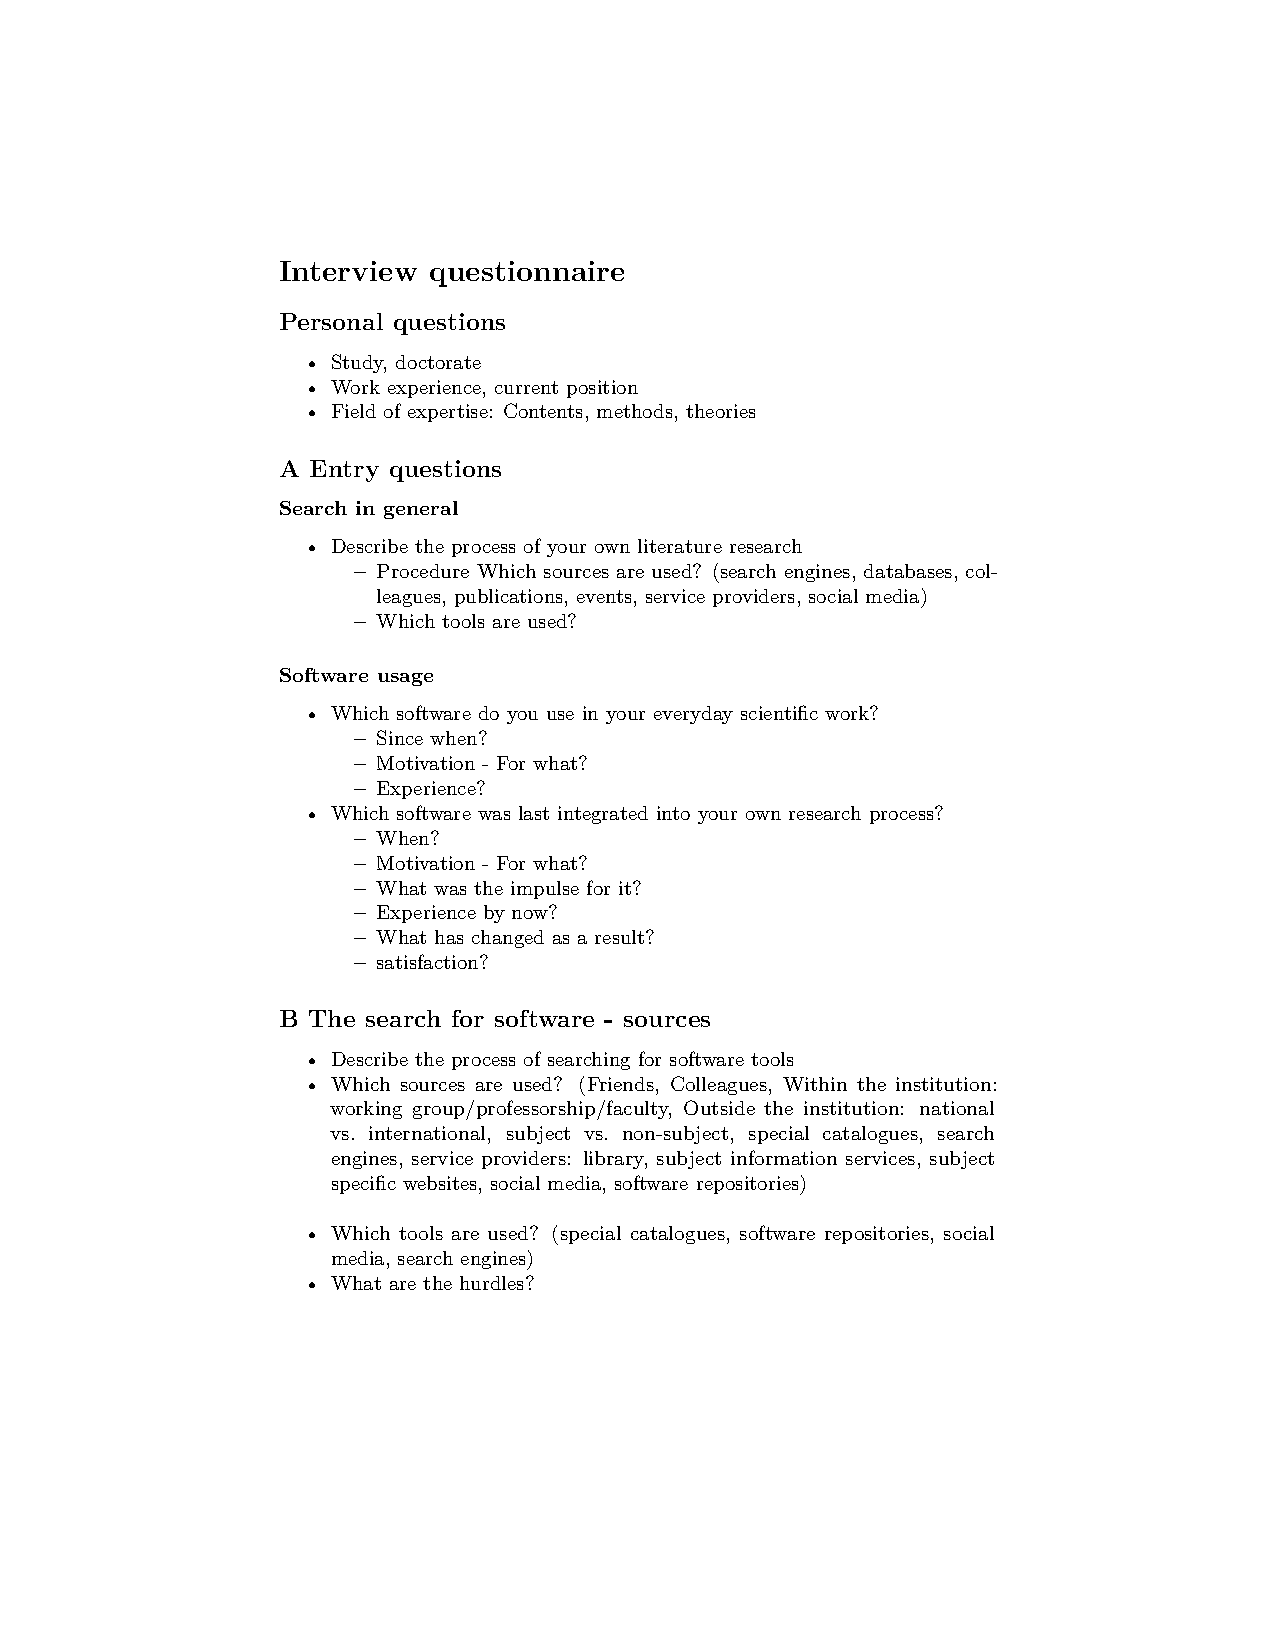
\includepdf[pages=-,pagecommand={\thispagestyle{empty}}]{_methods/Interview_guidelines_en.pdf}
\cleardoublepage

\chapter{Category System}
\label{sec:Category_system}
%\includepdf[pages=-,pagecommand={\thispagestyle{empty}}]{_analysis/....pdf}
\cleardoublepage

\chapter{Consent Form}
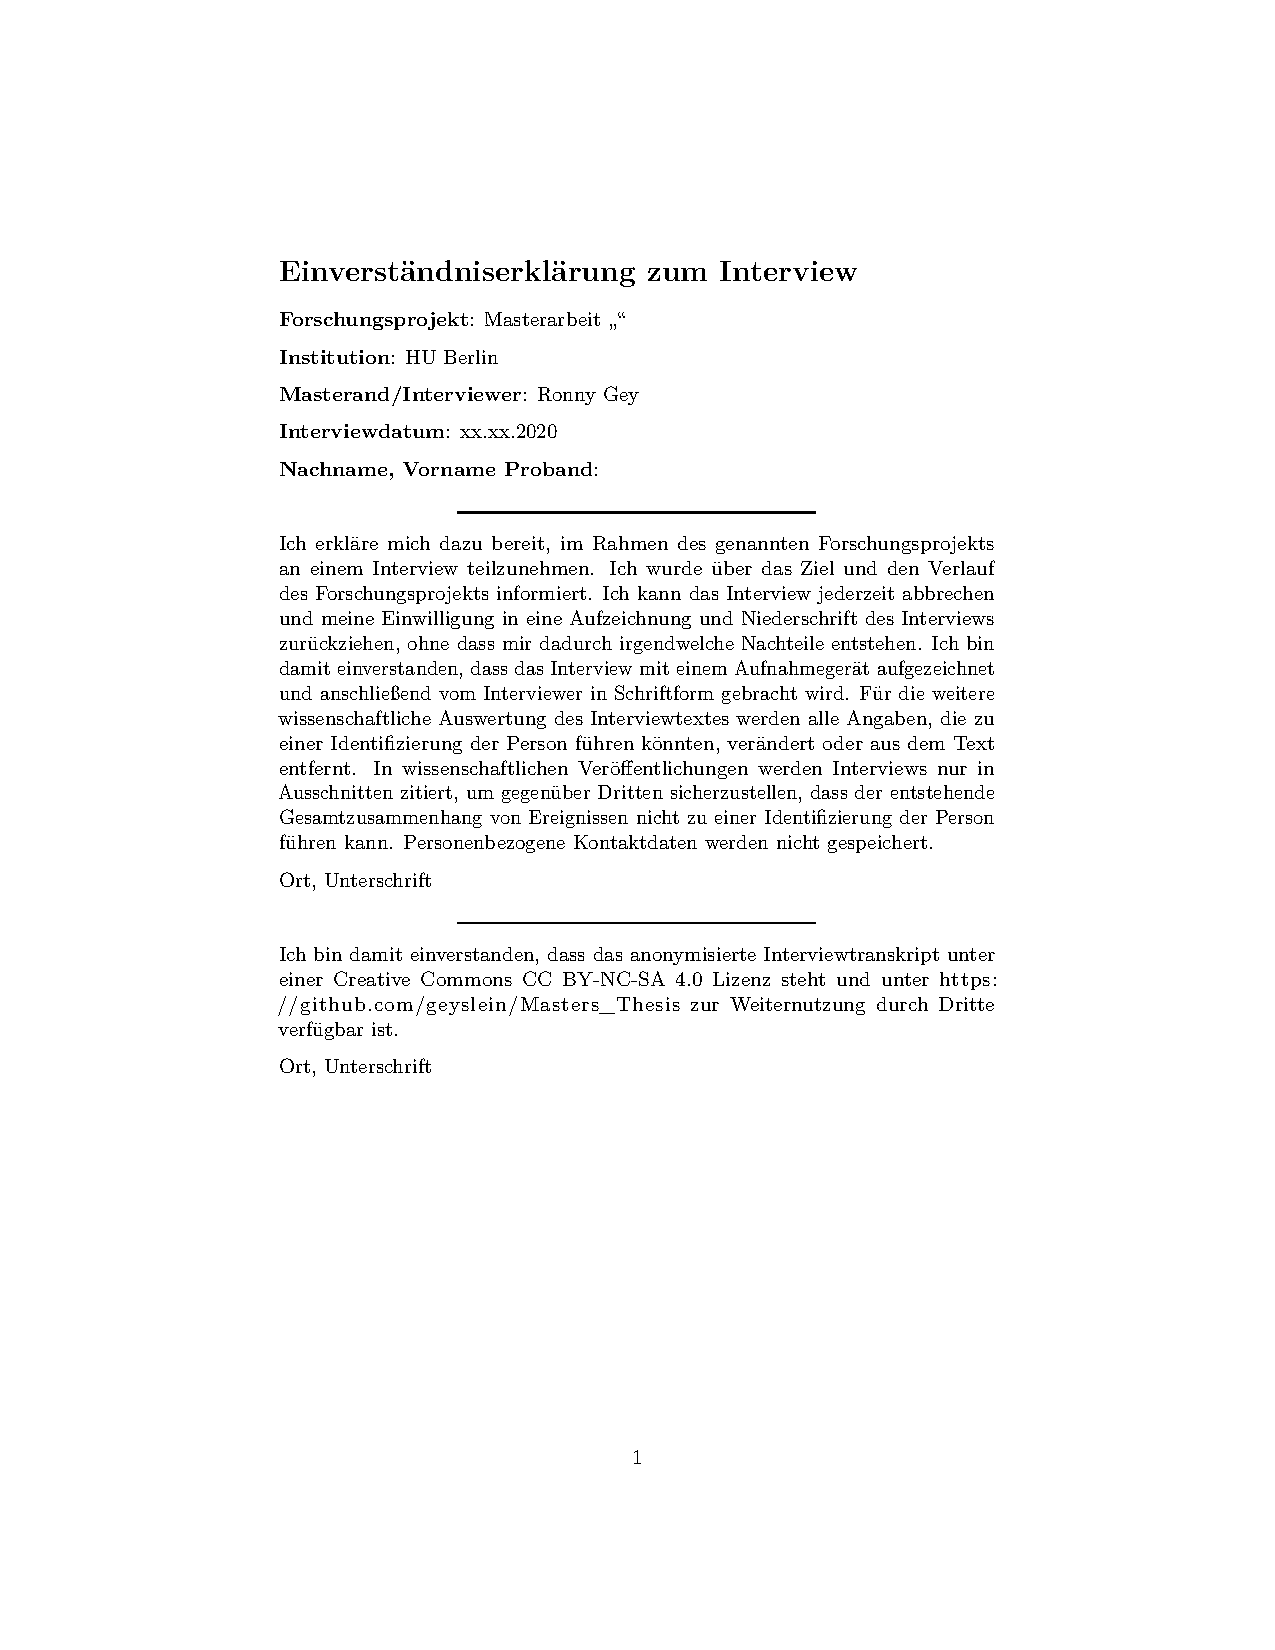
\includepdf[pages=-,pagecommand={\thispagestyle{empty}}]{_data/collection/consent form interview (German).pdf}

\end{appendices}
%======================================================================
%	Selbstständikeitserklärung
%======================================================================
\includepdf[pages=-,pagecommand={\thispagestyle{empty}}]{_admin/Selbststaendigkeitserklaerung}
\cleardoublepage

\end{document}